\documentclass[a4paper,11pt]{ctexbook}
\usepackage{mypreamble}
\begin{document}
\setcounter{chapter}{6}
\chapter{快速排序}
对于包含$ n $个数的输入数组来说,快速排序是一种最坏情况时间复杂度为$ \Theta(n^2) $的排序算法。虽然最坏情况时间复杂度很差,但是快速排序通常是实际排序应用中最好的选择,因为它的平均性能非常好:它的期望时间复杂度是$ \Theta(nlgn) $,而且$ \Theta(nlgn) $中隐含的常数因子非常小。另外它还能进行原址排序。
\section{快速排序的描述}
\begin{codebox}
	\Procname{$ \proc{QUICKSORT}(A,p,r) $}
	\li \If$ p < r $
	\li \Then 
	$ q = \proc{PARTITION}(A,p,r) $
	\li $ \proc{QUICKSORT}(A,p,q-1)$
	\li $ \proc{QUICKSORT}(A,q+1,r)$
	\End
\end{codebox}
\begin{codebox}
	\Procname{$ \proc{PARTITION}(A,p,r)$}
	\li $ \id{x} \gets A[r] $
	\li $ \id{i} \gets p-1 $
	\li \For$ \id{j} \gets p \To r-1 $
	\li \Do
	\If $ A[j] \leq x $
	\li 		\Then
	$ \id{i} \gets i+1 $
	\li 			exchange  $ A[i]$ with $A[j]$
	\End
	\End
	\li exchange $A[i+1]$ with $A[r] $
	\li \Return $ i+1 $
\end{codebox}
\section{快速排序的性能}
快速排序的运行时间依赖于划分是否平衡,而平衡与否又依赖于用于划分的元素。如果划分是平衡的,那么快速排序算法的性能与归并排序一样,否则就接近于 插入排序了。本节给出划分平衡或不平衡时快速排序性能的非形式化的分析。

\textbf{最坏情况划分}

当划分产生的连个子问题分别包含了$ n-1 $个元素和$ 0 $个元素时,快速排序的最坏情况发生了(当元素已按排好序)。不妨假设算法的每一次递归都出现了这种不平衡划分。划分操作的时间复杂度是$ \Theta(n) $。由于对一个大小为0的数组进行递归调用会直接返回,因此$ T(0) = \Theta(1) $,于是算法运行时间的递归表达式可以表示为:
\[
	T(n) = T(n-1) + T(0) + \Theta(n)
\]
从直观上来看,每一层递归的代价可以被累加起来,从而得到一个算术级数(公式(A.2)):
\[
	\sum_{k=1}^{n}k=\frac{1}{2}n(n+1)=\Theta(n^2)
\]
其结果为$ \Theta(n^2) $(如果这里没有理解到,试着画出其递归树就知道了)。实际上,利用代入法可以直接得到递归式$ T(n)=T(n-1)+\Theta(n) $的解为$ T(n)=\Theta(n^2) $。

因此,如果在算法的每一层递归上,划分都是最大程度不平衡的,那么算法的时间复杂度就是$ \Theta(n^2) $。也就是说,在最坏情况下,快速排序的运行时间并不比插入排序更好。此外,当输入数组已经完全有序时,快速排序的时间复杂度仍然为$ \Theta(n^2) $。而在同样情况下,插入排序的时间复杂度为$ O(n) $。

\textbf{最好情况的划分}

在可能的最平衡的划分中,$ \proc{PARTITION} $得到的两个子问题的规模都不大于$ n/2 $。这是因为其中一个子问题的规模为$ \floor{n/2} $。而另一个子问题的规模为$ \ceiling{n/2}-1 $。在这种情况下,快速排序的性能非常好。此时,算法运行时间的递归式为:
\[
	T(n)=2T(n/2)+\Theta(n)
\]
在上式中,我们忽略了一些余项以及减1的影响。根据主定理(定理4.1)的情况2,上述递归式的解为$ T(n)=\Theta(nlgn) $。

\textbf{平衡的划分}

快速排序的平均运行时间更接近于其最好情况,而非最坏情况。理解这一点的关键就是理解划分的平衡性是如何反映到描述运行时间的递归式上的。假设划分总是产生$ 9:1 $的划分,乍一看,这种划分是不平衡的。此时,我们得到的快速排序的时间复杂度的递归式为:
\[
	T(n) = T(9n/10) + T(n/10)+cn
\]
下图显示了这一递归调用所对应的递归树。注意,树中每一层的代价都是$ cn $,直到在深度$ \log_{10}{n}=\Theta(lgn) $处达到递归的边界条件为止,之后每层代价至多为$ cn $。递归在深度为$\log_{10/9}{n}=\Theta(n) $处终止。因此,快速排序的总代价为$ O(nlgn) $。因此,即使在递归的每一层上都是$ 9:1 $的划分,直观上看起来非常不平衡,但快速排序的运行时间是$ O(nlgn) $。\textbf{事实上,任何一种常数比例的划分都会产生深度为$ \Theta(lgn) $的递归树,其中每一层的时间代价都是$ O(n) $。因此,只要划分是常数比例的,算法的运行时间总是$ O(nlgn) $}。

\begin{figure}[htbp]	
	\begin{center}
	 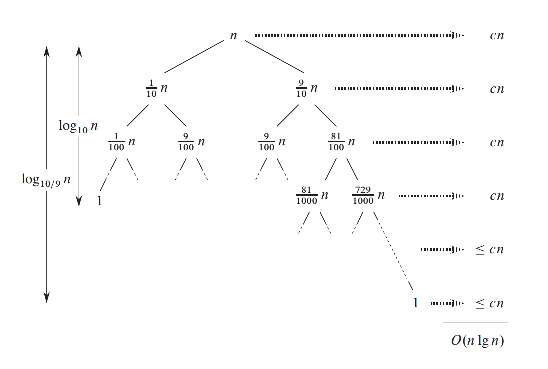
\includegraphics{figure/7.4.eps}	
	 \caption{$ \proc{QUICKSORT} $的一棵递归树,其中$ \proc{PARTITION} $总是产生$ 9:1 $的划分。该树的时间复杂度为$ O(nlgn) $。每个结点的值表示子问题的规模,每一层的代价显示在最右边。每一层的代价包含了$ \Theta(n) $项中隐含的常数}
	\end{center}	
\end{figure}

\section{快速排序的随机化版本}
在讨论快速排序的平均情况性能的时候,我们的前提假设是:输入数据的所有排列都是等概率的。但是在实际工程中,这个假设并不会总是成立。有时,我们可以通过在算法中引入随机性,从而使得算法对于所有的输入都能获得较好的期望性能。很多人都选择随机化版本的快速排序作为大数据输入情况下的排序算法。

在5.3节中,我们通过显式地对输入进行重新排列,使得算法实现随机化。当然,对于快速排序我们也可以这么做。但如果采用一种称为\textbf{随机抽样}(random sampling)的随机化技术,那么可以使得分析变得更加简单。与始终采用$ A[r] $作为主元的方法不同,随机抽样是从子数组$ A[p..r] $中随机选择一个元素作为主元。为达到这一目的,首先将$ A[r] $与从$ A[p..r] $中随机选出的一个元素交换。通过对序列$ p,\cdots,r $的随机抽样,可以保证主元元素$ x=A[r] $是等概率地从子数组的$ r-p+1 $个元素中选取的。因为主元是随机选取的,我们期望在平均情况下,对输入数组的划分是比较均衡的。
\begin{codebox}
	\Procname{$ \proc{RANDOMIZED-PARTITION}(A,p,r)$}
	\li $ \id{i} \gets \proc{RANDOM}(p,r)$
	\li exchange $ A[r] $ with $ A[i] $
	\li \Return $ \proc{PARTITION}(A,p,r) $
\end{codebox}
\begin{codebox}
	\Procname{$ \proc{RANDOMIZED-QUICKSORT}(A,p,r)$}
	\li \If $ p<r $
	\li \Then
		 $q\gets \proc{RANDOMIZED-PARTITION}(A,p,r) $
	\li	 $\proc{RANDOMIZED-QUICKSORT(A,p,q-1)} $
	\li  $\proc{RANDOMIZED-QUICKSORT(A,q+1,r)} $	
		\End 
\end{codebox}

\end{document}
